\documentclass[1p]{elsarticle_modified}
%\bibliographystyle{elsarticle-num}

%\usepackage[colorlinks]{hyperref}
%\usepackage{abbrmath_seonhwa} %\Abb, \Ascr, \Acal ,\Abf, \Afrak
\usepackage{amsfonts}
\usepackage{amssymb}
\usepackage{amsmath}
\usepackage{amsthm}
\usepackage{scalefnt}
\usepackage{amsbsy}
\usepackage{kotex}
\usepackage{caption}
\usepackage{subfig}
\usepackage{color}
\usepackage{graphicx}
\usepackage{xcolor} %% white, black, red, green, blue, cyan, magenta, yellow
\usepackage{float}
\usepackage{setspace}
\usepackage{hyperref}

\usepackage{tikz}
\usetikzlibrary{arrows}

\usepackage{multirow}
\usepackage{array} % fixed length table
\usepackage{hhline}

%%%%%%%%%%%%%%%%%%%%%
\makeatletter
\renewcommand*\env@matrix[1][\arraystretch]{%
	\edef\arraystretch{#1}%
	\hskip -\arraycolsep
	\let\@ifnextchar\new@ifnextchar
	\array{*\c@MaxMatrixCols c}}
\makeatother %https://tex.stackexchange.com/questions/14071/how-can-i-increase-the-line-spacing-in-a-matrix
%%%%%%%%%%%%%%%

\usepackage[normalem]{ulem}

\newcommand{\msout}[1]{\ifmmode\text{\sout{\ensuremath{#1}}}\else\sout{#1}\fi}
%SOURCE: \msout is \stkout macro in https://tex.stackexchange.com/questions/20609/strikeout-in-math-mode

\newcommand{\cancel}[1]{
	\ifmmode
	{\color{red}\msout{#1}}
	\else
	{\color{red}\sout{#1}}
	\fi
}

\newcommand{\add}[1]{
	{\color{blue}\uwave{#1}}
}

\newcommand{\replace}[2]{
	\ifmmode
	{\color{red}\msout{#1}}{\color{blue}\uwave{#2}}
	\else
	{\color{red}\sout{#1}}{\color{blue}\uwave{#2}}
	\fi
}

\newcommand{\Sol}{\mathcal{S}} %segment
\newcommand{\D}{D} %diagram
\newcommand{\A}{\mathcal{A}} %arc


%%%%%%%%%%%%%%%%%%%%%%%%%%%%%5 test

\def\sl{\operatorname{\textup{SL}}(2,\Cbb)}
\def\psl{\operatorname{\textup{PSL}}(2,\Cbb)}
\def\quan{\mkern 1mu \triangleright \mkern 1mu}

\theoremstyle{definition}
\newtheorem{thm}{Theorem}[section]
\newtheorem{prop}[thm]{Proposition}
\newtheorem{lem}[thm]{Lemma}
\newtheorem{ques}[thm]{Question}
\newtheorem{cor}[thm]{Corollary}
\newtheorem{defn}[thm]{Definition}
\newtheorem{exam}[thm]{Example}
\newtheorem{rmk}[thm]{Remark}
\newtheorem{alg}[thm]{Algorithm}

\newcommand{\I}{\sqrt{-1}}
\begin{document}

%\begin{frontmatter}
%
%\title{Boundary parabolic representations of knots up to 8 crossings}
%
%%% Group authors per affiliation:
%\author{Yunhi Cho} 
%\address{Department of Mathematics, University of Seoul, Seoul, Korea}
%\ead{yhcho@uos.ac.kr}
%
%
%\author{Seonhwa Kim} %\fnref{s_kim}}
%\address{Center for Geometry and Physics, Institute for Basic Science, Pohang, 37673, Korea}
%\ead{ryeona17@ibs.re.kr}
%
%\author{Hyuk Kim}
%\address{Department of Mathematical Sciences, Seoul National University, Seoul 08826, Korea}
%\ead{hyukkim@snu.ac.kr}
%
%\author{Seokbeom Yoon}
%\address{Department of Mathematical Sciences, Seoul National University, Seoul, 08826,  Korea}
%\ead{sbyoon15@snu.ac.kr}
%
%\begin{abstract}
%We find all boundary parabolic representation of knots up to 8 crossings.
%
%\end{abstract}
%\begin{keyword}
%    \MSC[2010] 57M25 
%\end{keyword}
%
%\end{frontmatter}

%\linenumbers
%\tableofcontents
%
\newcommand\colored[1]{\textcolor{white}{\rule[-0.35ex]{0.8em}{1.4ex}}\kern-0.8em\color{red} #1}%
%\newcommand\colored[1]{\textcolor{white}{ #1}\kern-2.17ex	\textcolor{white}{ #1}\kern-1.81ex	\textcolor{white}{ #1}\kern-2.15ex\color{red}#1	}

{\Large $\underline{12n_{0830}~(K12n_{0830})}$}

\setlength{\tabcolsep}{10pt}
\renewcommand{\arraystretch}{1.6}
\vspace{1cm}\begin{tabular}{m{100pt}>{\centering\arraybackslash}m{274pt}}
\multirow{5}{120pt}{
	\centering
	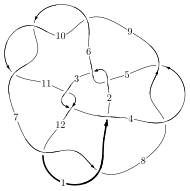
\includegraphics[width=112pt]{../../../GIT/diagram.site/Diagrams/png/2919_12n_0830.png}\\
\ \ \ A knot diagram\footnotemark}&
\allowdisplaybreaks
\textbf{Linearized knot diagam} \\
\cline{2-2}
 &
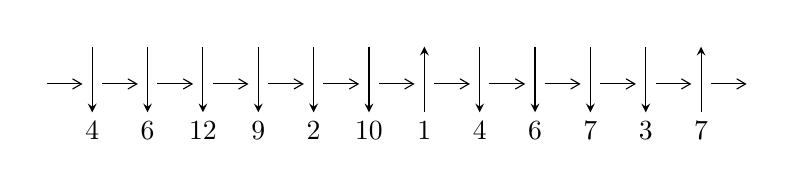
\begin{tikzpicture}[x=20pt, y=17pt]
	% nodes
	\node (C0) at (0, 0) {};
	\node (C1) at (1, 0) {};
	\node (C1U) at (1, +1) {};
	\node (C1D) at (1, -1) {4};

	\node (C2) at (2, 0) {};
	\node (C2U) at (2, +1) {};
	\node (C2D) at (2, -1) {6};

	\node (C3) at (3, 0) {};
	\node (C3U) at (3, +1) {};
	\node (C3D) at (3, -1) {12};

	\node (C4) at (4, 0) {};
	\node (C4U) at (4, +1) {};
	\node (C4D) at (4, -1) {9};

	\node (C5) at (5, 0) {};
	\node (C5U) at (5, +1) {};
	\node (C5D) at (5, -1) {2};

	\node (C6) at (6, 0) {};
	\node (C6U) at (6, +1) {};
	\node (C6D) at (6, -1) {10};

	\node (C7) at (7, 0) {};
	\node (C7U) at (7, +1) {};
	\node (C7D) at (7, -1) {1};

	\node (C8) at (8, 0) {};
	\node (C8U) at (8, +1) {};
	\node (C8D) at (8, -1) {4};

	\node (C9) at (9, 0) {};
	\node (C9U) at (9, +1) {};
	\node (C9D) at (9, -1) {6};

	\node (C10) at (10, 0) {};
	\node (C10U) at (10, +1) {};
	\node (C10D) at (10, -1) {7};

	\node (C11) at (11, 0) {};
	\node (C11U) at (11, +1) {};
	\node (C11D) at (11, -1) {3};

	\node (C12) at (12, 0) {};
	\node (C12U) at (12, +1) {};
	\node (C12D) at (12, -1) {7};
	\node (C13) at (13, 0) {};

	% arrows
	\draw[->,>={angle 60}]
	(C0) edge (C1) (C1) edge (C2) (C2) edge (C3) (C3) edge (C4) (C4) edge (C5) (C5) edge (C6) (C6) edge (C7) (C7) edge (C8) (C8) edge (C9) (C9) edge (C10) (C10) edge (C11) (C11) edge (C12) (C12) edge (C13) ;	\draw[->,>=stealth]
	(C1U) edge (C1D) (C2U) edge (C2D) (C3U) edge (C3D) (C4U) edge (C4D) (C5U) edge (C5D) (C6U) edge (C6D) (C7D) edge (C7U) (C8U) edge (C8D) (C9U) edge (C9D) (C10U) edge (C10D) (C11U) edge (C11D) (C12D) edge (C12U) ;
	\end{tikzpicture} \\
\hhline{~~} \\& 
\textbf{Solving Sequence} \\ \cline{2-2} 
 &
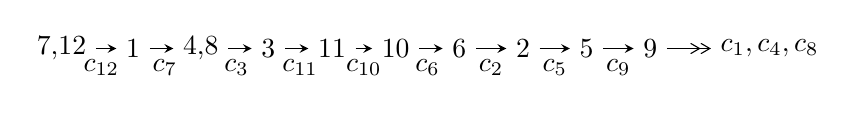
\begin{tikzpicture}[x=23pt, y=7pt]
	% node
	\node (A0) at (-1/8, 0) {7,12};
	\node (A1) at (1, 0) {1};
	\node (A2) at (33/16, 0) {4,8};
	\node (A3) at (25/8, 0) {3};
	\node (A4) at (33/8, 0) {11};
	\node (A5) at (41/8, 0) {10};
	\node (A6) at (49/8, 0) {6};
	\node (A7) at (57/8, 0) {2};
	\node (A8) at (65/8, 0) {5};
	\node (A9) at (73/8, 0) {9};
	\node (C1) at (1/2, -1) {$c_{12}$};
	\node (C2) at (3/2, -1) {$c_{7}$};
	\node (C3) at (21/8, -1) {$c_{3}$};
	\node (C4) at (29/8, -1) {$c_{11}$};
	\node (C5) at (37/8, -1) {$c_{10}$};
	\node (C6) at (45/8, -1) {$c_{6}$};
	\node (C7) at (53/8, -1) {$c_{2}$};
	\node (C8) at (61/8, -1) {$c_{5}$};
	\node (C9) at (69/8, -1) {$c_{9}$};
	\node (A10) at (11, 0) {$c_{1},c_{4},c_{8}$};

	% edge
	\draw[->,>=stealth]	
	(A0) edge (A1) (A1) edge (A2) (A2) edge (A3) (A3) edge (A4) (A4) edge (A5) (A5) edge (A6) (A6) edge (A7) (A7) edge (A8) (A8) edge (A9) ;
	\draw[->>,>={angle 60}]	
	(A9) edge (A10);
\end{tikzpicture} \\ 

\end{tabular} \\

\footnotetext{
The image of knot diagram is generated by the software ``\textbf{Draw programme}" developed by Andrew Bartholomew(\url{http://www.layer8.co.uk/maths/draw/index.htm\#Running-draw}), where we modified some parts for our purpose(\url{https://github.com/CATsTAILs/LinksPainter}).
}\phantom \\ \newline 
\centering \textbf{Ideals for irreducible components\footnotemark of $X_{\text{par}}$} 
 
\begin{align*}
I^u_{1}&=\langle 
7 u^{11}-9 u^{10}-37 u^9+25 u^8+84 u^7-6 u^6-54 u^5-45 u^4-53 u^3+27 u^2+11 b+46 u+9,\\
\phantom{I^u_{1}}&\phantom{= \langle  }10 u^{11}-38 u^{10}-12 u^9+152 u^8-12 u^7-249 u^6+36 u^5+85 u^4+6 u^3+180 u^2+11 a-82 u-83,\\
\phantom{I^u_{1}}&\phantom{= \langle  }u^{12}-4 u^{11}+15 u^9-6 u^8-24 u^7+11 u^6+8 u^5+17 u^3-14 u^2-6 u+1\rangle \\
I^u_{2}&=\langle 
u^3+2 u^2+b,\;u^2+a+u-1,\;u^4+3 u^3+2 u^2+1\rangle \\
I^u_{3}&=\langle 
u^2+b+a+u-2,\;2 u^2 a+a^2+a u- u^2-4 a- u+4,\;u^3+u^2-2 u-1\rangle \\
I^u_{4}&=\langle 
- u^2+b+a+u+2,\;-2 u^2 a+a^2+a u- u^2+4 a+u+2,\;u^3- u^2-2 u+1\rangle \\
\\
\end{align*}
\raggedright * 4 irreducible components of $\dim_{\mathbb{C}}=0$, with total 28 representations.\\
\footnotetext{All coefficients of polynomials are rational numbers. But the coefficients are sometimes approximated in decimal forms when there is not enough margin.}
\newpage
\renewcommand{\arraystretch}{1}
\centering \section*{I. $I^u_{1}= \langle 7 u^{11}-9 u^{10}+\cdots+11 b+9,\;10 u^{11}-38 u^{10}+\cdots+11 a-83,\;u^{12}-4 u^{11}+\cdots-6 u+1 \rangle$}
\flushleft \textbf{(i) Arc colorings}\\
\begin{tabular}{m{7pt} m{180pt} m{7pt} m{180pt} }
\flushright $a_{7}=$&$\begin{pmatrix}0\\u\end{pmatrix}$ \\
\flushright $a_{12}=$&$\begin{pmatrix}1\\0\end{pmatrix}$ \\
\flushright $a_{1}=$&$\begin{pmatrix}1\\- u^2\end{pmatrix}$ \\
\flushright $a_{4}=$&$\begin{pmatrix}-0.909091 u^{11}+3.45455 u^{10}+\cdots+7.45455 u+7.54545\\-0.636364 u^{11}+0.818182 u^{10}+\cdots-4.18182 u-0.818182\end{pmatrix}$ \\
\flushright $a_{8}=$&$\begin{pmatrix}u\\- u^3+u\end{pmatrix}$ \\
\flushright $a_{3}=$&$\begin{pmatrix}-1.54545 u^{11}+4.27273 u^{10}+\cdots+3.27273 u+6.72727\\-0.636364 u^{11}+0.818182 u^{10}+\cdots-4.18182 u-0.818182\end{pmatrix}$ \\
\flushright $a_{11}=$&$\begin{pmatrix}-0.818182 u^{11}+3.90909 u^{10}+\cdots+13.9091 u+9.09091\\0.545455 u^{11}-1.27273 u^{10}+\cdots-2.27273 u-1.72727\end{pmatrix}$ \\
\flushright $a_{10}=$&$\begin{pmatrix}-0.818182 u^{11}+3.90909 u^{10}+\cdots+13.9091 u+9.09091\\-1.18182 u^{11}+2.09091 u^{10}+\cdots-6.90909 u-1.09091\end{pmatrix}$ \\
\flushright $a_{6}=$&$\begin{pmatrix}-1.72727 u^{11}+6.36364 u^{10}+\cdots+20.3636 u+12.6364\\2.81818 u^{11}-6.90909 u^{10}+\cdots+5.09091 u-4.09091\end{pmatrix}$ \\
\flushright $a_{2}=$&$\begin{pmatrix}2.72727 u^{11}-8.36364 u^{10}+\cdots-10.3636 u-8.63636\\-0.0909091 u^{11}+0.545455 u^{10}+\cdots+2.54545 u+1.45455\end{pmatrix}$ \\
\flushright $a_{5}=$&$\begin{pmatrix}-5.63636 u^{11}+12.8182 u^{10}+\cdots-5.18182 u+6.18182\\10.6364 u^{11}-24.8182 u^{10}+\cdots+33.1818 u-7.18182\end{pmatrix}$ \\
\flushright $a_{9}=$&$\begin{pmatrix}2.72727 u^{11}-8.36364 u^{10}+\cdots-9.36364 u-9.63636\\-0.0909091 u^{11}+0.545455 u^{10}+\cdots+3.54545 u+1.45455\end{pmatrix}$\\&\end{tabular}
\flushleft \textbf{(ii) Obstruction class $= -1$}\\~\\
\flushleft \textbf{(iii) Cusp Shapes $= -\frac{5}{11} u^{11}-\frac{14}{11} u^{10}+\frac{72}{11} u^9+\frac{67}{11} u^8-\frac{225}{11} u^7-\frac{189}{11} u^6+\frac{224}{11} u^5+\frac{194}{11} u^4+\frac{151}{11} u^3+\frac{53}{11} u^2-\frac{278}{11} u-\frac{206}{11}$}\\~\\
\newpage\renewcommand{\arraystretch}{1}
\flushleft \textbf{(iv) u-Polynomials at the component}\newline \\
\begin{tabular}{m{50pt}|m{274pt}}
Crossings & \hspace{64pt}u-Polynomials at each crossing \\
\hline $$\begin{aligned}c_{1},c_{4},c_{8}\end{aligned}$$&$\begin{aligned}
&u^{12}- u^{11}+\cdots+3 u+1
\end{aligned}$\\
\hline $$\begin{aligned}c_{2},c_{5}\end{aligned}$$&$\begin{aligned}
&u^{12}+6 u^{10}+\cdots+6 u-1
\end{aligned}$\\
\hline $$\begin{aligned}c_{3},c_{6},c_{9}\\c_{10},c_{11}\end{aligned}$$&$\begin{aligned}
&u^{12}+2 u^{11}+\cdots-5 u-1
\end{aligned}$\\
\hline $$\begin{aligned}c_{7},c_{12}\end{aligned}$$&$\begin{aligned}
&u^{12}-4 u^{11}+15 u^9-6 u^8-24 u^7+11 u^6+8 u^5+17 u^3-14 u^2-6 u+1
\end{aligned}$\\
\hline
\end{tabular}\\~\\
\newpage\renewcommand{\arraystretch}{1}
\flushleft \textbf{(v) Riley Polynomials at the component}\newline \\
\begin{tabular}{m{50pt}|m{274pt}}
Crossings & \hspace{64pt}Riley Polynomials at each crossing \\
\hline $$\begin{aligned}c_{1},c_{4},c_{8}\end{aligned}$$&$\begin{aligned}
&y^{12}+21 y^{11}+\cdots+7 y+1
\end{aligned}$\\
\hline $$\begin{aligned}c_{2},c_{5}\end{aligned}$$&$\begin{aligned}
&y^{12}+12 y^{11}+\cdots-24 y+1
\end{aligned}$\\
\hline $$\begin{aligned}c_{3},c_{6},c_{9}\\c_{10},c_{11}\end{aligned}$$&$\begin{aligned}
&y^{12}-10 y^{11}+\cdots-27 y+1
\end{aligned}$\\
\hline $$\begin{aligned}c_{7},c_{12}\end{aligned}$$&$\begin{aligned}
&y^{12}-16 y^{11}+\cdots-64 y+1
\end{aligned}$\\
\hline
\end{tabular}\\~\\
\newpage\flushleft \textbf{(vi) Complex Volumes and Cusp Shapes}
$$\begin{array}{c|c|c}  
\text{Solutions to }I^u_{1}& \I (\text{vol} + \sqrt{-1}CS) & \text{Cusp shape}\\
 \hline 
\begin{aligned}
u &= \phantom{-}1.10971\phantom{ +0.000000I} \\
a &= \phantom{-}0.161640\phantom{ +0.000000I} \\
b &= \phantom{-}1.43592\phantom{ +0.000000I}\end{aligned}
 & -8.31956\phantom{ +0.000000I} & -9.86310\phantom{ +0.000000I} \\ \hline\begin{aligned}
u &= -0.047522 + 0.875928 I \\
a &= \phantom{-}0.550543 - 0.109390 I \\
b &= \phantom{-}0.620121 - 0.344417 I\end{aligned}
 & -0.93869 + 1.18818 I & -6.72604 - 6.20651 I \\ \hline\begin{aligned}
u &= -0.047522 - 0.875928 I \\
a &= \phantom{-}0.550543 + 0.109390 I \\
b &= \phantom{-}0.620121 + 0.344417 I\end{aligned}
 & -0.93869 - 1.18818 I & -6.72604 + 6.20651 I \\ \hline\begin{aligned}
u &= -1.25634\phantom{ +0.000000I} \\
a &= -1.19132\phantom{ +0.000000I} \\
b &= \phantom{-}1.21703\phantom{ +0.000000I}\end{aligned}
 & -6.81354\phantom{ +0.000000I} & -13.0130\phantom{ +0.000000I} \\ \hline\begin{aligned}
u &= -1.235650 + 0.562992 I \\
a &= -0.167466 + 0.934549 I \\
b &= -1.095690 - 0.804498 I\end{aligned}
 & \phantom{-}3.14055 - 6.45902 I & -9.32911 + 6.09999 I \\ \hline\begin{aligned}
u &= -1.235650 - 0.562992 I \\
a &= -0.167466 - 0.934549 I \\
b &= -1.095690 + 0.804498 I\end{aligned}
 & \phantom{-}3.14055 + 6.45902 I & -9.32911 - 6.09999 I \\ \hline\begin{aligned}
u &= -0.405006\phantom{ +0.000000I} \\
a &= \phantom{-}1.79428\phantom{ +0.000000I} \\
b &= \phantom{-}0.222902\phantom{ +0.000000I}\end{aligned}
 & -0.968428\phantom{ +0.000000I} & -8.39760\phantom{ +0.000000I} \\ \hline\begin{aligned}
u &= \phantom{-}1.68726 + 0.16814 I \\
a &= \phantom{-}0.086359 - 0.758415 I \\
b &= -0.723528 + 0.260031 I\end{aligned}
 & \phantom{-}5.78393 + 2.23624 I & -8.95764 - 2.44896 I \\ \hline\begin{aligned}
u &= \phantom{-}1.68726 - 0.16814 I \\
a &= \phantom{-}0.086359 + 0.758415 I \\
b &= -0.723528 - 0.260031 I\end{aligned}
 & \phantom{-}5.78393 - 2.23624 I & -8.95764 + 2.44896 I \\ \hline\begin{aligned}
u &= \phantom{-}1.80553 + 0.13825 I \\
a &= -0.47270 + 1.37792 I \\
b &= \phantom{-}1.46230 - 1.09221 I\end{aligned}
 & \phantom{-}14.0244 + 9.4961 I & -8.37495 - 3.79641 I\\
 \hline 
 \end{array}$$\newpage$$\begin{array}{c|c|c}  
\text{Solutions to }I^u_{1}& \I (\text{vol} + \sqrt{-1}CS) & \text{Cusp shape}\\
 \hline 
\begin{aligned}
u &= \phantom{-}1.80553 - 0.13825 I \\
a &= -0.47270 - 1.37792 I \\
b &= \phantom{-}1.46230 + 1.09221 I\end{aligned}
 & \phantom{-}14.0244 - 9.4961 I & -8.37495 + 3.79641 I \\ \hline\begin{aligned}
u &= \phantom{-}0.132401\phantom{ +0.000000I} \\
a &= \phantom{-}8.24194\phantom{ +0.000000I} \\
b &= -1.40225\phantom{ +0.000000I}\end{aligned}
 & -11.4695\phantom{ +0.000000I} & -21.9510\phantom{ +0.000000I}\\
 \hline 
 \end{array}$$\newpage\newpage\renewcommand{\arraystretch}{1}
\centering \section*{II. $I^u_{2}= \langle u^3+2 u^2+b,\;u^2+a+u-1,\;u^4+3 u^3+2 u^2+1 \rangle$}
\flushleft \textbf{(i) Arc colorings}\\
\begin{tabular}{m{7pt} m{180pt} m{7pt} m{180pt} }
\flushright $a_{7}=$&$\begin{pmatrix}0\\u\end{pmatrix}$ \\
\flushright $a_{12}=$&$\begin{pmatrix}1\\0\end{pmatrix}$ \\
\flushright $a_{1}=$&$\begin{pmatrix}1\\- u^2\end{pmatrix}$ \\
\flushright $a_{4}=$&$\begin{pmatrix}- u^2- u+1\\- u^3-2 u^2\end{pmatrix}$ \\
\flushright $a_{8}=$&$\begin{pmatrix}u\\- u^3+u\end{pmatrix}$ \\
\flushright $a_{3}=$&$\begin{pmatrix}- u^3-3 u^2- u+1\\- u^3-2 u^2\end{pmatrix}$ \\
\flushright $a_{11}=$&$\begin{pmatrix}u^2+2 u\\- u^3- u^2+u-1\end{pmatrix}$ \\
\flushright $a_{10}=$&$\begin{pmatrix}u^2+2 u\\u^2+u\end{pmatrix}$ \\
\flushright $a_{6}=$&$\begin{pmatrix}- u^3-2 u^2- u-1\\0\end{pmatrix}$ \\
\flushright $a_{2}=$&$\begin{pmatrix}- u^3-2 u^2+1\\- u^3-2 u^2\end{pmatrix}$ \\
\flushright $a_{5}=$&$\begin{pmatrix}- u^3-2 u^2\\u^3+u^2+1\end{pmatrix}$ \\
\flushright $a_{9}=$&$\begin{pmatrix}u^3+2 u^2+u\\u^2+u\end{pmatrix}$\\&\end{tabular}
\flushleft \textbf{(ii) Obstruction class $= 1$}\\~\\
\flushleft \textbf{(iii) Cusp Shapes $= 4 u^3+5 u^2-5 u-13$}\\~\\
\newpage\renewcommand{\arraystretch}{1}
\flushleft \textbf{(iv) u-Polynomials at the component}\newline \\
\begin{tabular}{m{50pt}|m{274pt}}
Crossings & \hspace{64pt}u-Polynomials at each crossing \\
\hline $$\begin{aligned}c_{1},c_{4}\end{aligned}$$&$\begin{aligned}
&u^4+2 u^2-3 u+1
\end{aligned}$\\
\hline $$\begin{aligned}c_{2}\end{aligned}$$&$\begin{aligned}
&u^4- u^3+2 u^2-2 u+1
\end{aligned}$\\
\hline $$\begin{aligned}c_{3},c_{9},c_{10}\end{aligned}$$&$\begin{aligned}
&u^4- u^3- u^2+u+1
\end{aligned}$\\
\hline $$\begin{aligned}c_{5}\end{aligned}$$&$\begin{aligned}
&u^4+u^3+2 u^2+2 u+1
\end{aligned}$\\
\hline $$\begin{aligned}c_{6},c_{11}\end{aligned}$$&$\begin{aligned}
&u^4+u^3- u^2- u+1
\end{aligned}$\\
\hline $$\begin{aligned}c_{7}\end{aligned}$$&$\begin{aligned}
&u^4-3 u^3+2 u^2+1
\end{aligned}$\\
\hline $$\begin{aligned}c_{8}\end{aligned}$$&$\begin{aligned}
&u^4+2 u^2+3 u+1
\end{aligned}$\\
\hline $$\begin{aligned}c_{12}\end{aligned}$$&$\begin{aligned}
&u^4+3 u^3+2 u^2+1
\end{aligned}$\\
\hline
\end{tabular}\\~\\
\newpage\renewcommand{\arraystretch}{1}
\flushleft \textbf{(v) Riley Polynomials at the component}\newline \\
\begin{tabular}{m{50pt}|m{274pt}}
Crossings & \hspace{64pt}Riley Polynomials at each crossing \\
\hline $$\begin{aligned}c_{1},c_{4},c_{8}\end{aligned}$$&$\begin{aligned}
&y^4+4 y^3+6 y^2-5 y+1
\end{aligned}$\\
\hline $$\begin{aligned}c_{2},c_{5}\end{aligned}$$&$\begin{aligned}
&y^4+3 y^3+2 y^2+1
\end{aligned}$\\
\hline $$\begin{aligned}c_{3},c_{6},c_{9}\\c_{10},c_{11}\end{aligned}$$&$\begin{aligned}
&y^4-3 y^3+5 y^2-3 y+1
\end{aligned}$\\
\hline $$\begin{aligned}c_{7},c_{12}\end{aligned}$$&$\begin{aligned}
&y^4-5 y^3+6 y^2+4 y+1
\end{aligned}$\\
\hline
\end{tabular}\\~\\
\newpage\flushleft \textbf{(vi) Complex Volumes and Cusp Shapes}
$$\begin{array}{c|c|c}  
\text{Solutions to }I^u_{2}& \I (\text{vol} + \sqrt{-1}CS) & \text{Cusp shape}\\
 \hline 
\begin{aligned}
u &= \phantom{-}0.192440 + 0.547877 I \\
a &= \phantom{-}1.070700 - 0.758745 I \\
b &= \phantom{-}0.692440 - 0.318148 I\end{aligned}
 & -1.74699 + 0.56550 I & -15.9426 - 2.0994 I \\ \hline\begin{aligned}
u &= \phantom{-}0.192440 - 0.547877 I \\
a &= \phantom{-}1.070700 + 0.758745 I \\
b &= \phantom{-}0.692440 + 0.318148 I\end{aligned}
 & -1.74699 - 0.56550 I & -15.9426 + 2.0994 I \\ \hline\begin{aligned}
u &= -1.69244 + 0.31815 I \\
a &= -0.070696 + 0.758745 I \\
b &= -1.192440 - 0.547877 I\end{aligned}
 & \phantom{-}5.03685 - 4.62527 I & -8.05745 + 3.83145 I \\ \hline\begin{aligned}
u &= -1.69244 - 0.31815 I \\
a &= -0.070696 - 0.758745 I \\
b &= -1.192440 + 0.547877 I\end{aligned}
 & \phantom{-}5.03685 + 4.62527 I & -8.05745 - 3.83145 I\\
 \hline 
 \end{array}$$\newpage\newpage\renewcommand{\arraystretch}{1}
\centering \section*{III. $I^u_{3}= \langle u^2+b+a+u-2,\;2 u^2 a+a^2+a u- u^2-4 a- u+4,\;u^3+u^2-2 u-1 \rangle$}
\flushleft \textbf{(i) Arc colorings}\\
\begin{tabular}{m{7pt} m{180pt} m{7pt} m{180pt} }
\flushright $a_{7}=$&$\begin{pmatrix}0\\u\end{pmatrix}$ \\
\flushright $a_{12}=$&$\begin{pmatrix}1\\0\end{pmatrix}$ \\
\flushright $a_{1}=$&$\begin{pmatrix}1\\- u^2\end{pmatrix}$ \\
\flushright $a_{4}=$&$\begin{pmatrix}a\\- u^2- a- u+2\end{pmatrix}$ \\
\flushright $a_{8}=$&$\begin{pmatrix}u\\u^2- u-1\end{pmatrix}$ \\
\flushright $a_{3}=$&$\begin{pmatrix}- u^2- u+2\\- u^2- a- u+2\end{pmatrix}$ \\
\flushright $a_{11}=$&$\begin{pmatrix}- u^2 a- a u+2 u^2+2 a+u-4\\- a u+u^2-1\end{pmatrix}$ \\
\flushright $a_{10}=$&$\begin{pmatrix}- u^2 a- a u+2 u^2+2 a+u-4\\0\end{pmatrix}$ \\
\flushright $a_{6}=$&$\begin{pmatrix}- u^2- a- u+2\\u\end{pmatrix}$ \\
\flushright $a_{2}=$&$\begin{pmatrix}-3 u^2- a+5\\u^2 a- a- u+1\end{pmatrix}$ \\
\flushright $a_{5}=$&$\begin{pmatrix}-3 u^2 a+a u+u^2+2 a-4\\u^2 a- a u- u^2+3 u\end{pmatrix}$ \\
\flushright $a_{9}=$&$\begin{pmatrix}- u^2 a- a u+3 u^2+2 a+u-4\\a u- u^2+1\end{pmatrix}$\\&\end{tabular}
\flushleft \textbf{(ii) Obstruction class $= -1$}\\~\\
\flushleft \textbf{(iii) Cusp Shapes $= -7$}\\~\\
\newpage\renewcommand{\arraystretch}{1}
\flushleft \textbf{(iv) u-Polynomials at the component}\newline \\
\begin{tabular}{m{50pt}|m{274pt}}
Crossings & \hspace{64pt}u-Polynomials at each crossing \\
\hline $$\begin{aligned}c_{1},c_{4},c_{8}\end{aligned}$$&$\begin{aligned}
&u^6- u^5+12 u^4-6 u^3-7 u^2+7 u+7
\end{aligned}$\\
\hline $$\begin{aligned}c_{2},c_{5}\end{aligned}$$&$\begin{aligned}
&u^6+u^5+9 u^4+18 u^3+26 u^2+29 u+13
\end{aligned}$\\
\hline $$\begin{aligned}c_{3},c_{6},c_{9}\\c_{10},c_{11}\end{aligned}$$&$\begin{aligned}
&u^6+u^5+3 u^4+5 u^2+2 u+1
\end{aligned}$\\
\hline $$\begin{aligned}c_{7},c_{12}\end{aligned}$$&$\begin{aligned}
&(u^3+u^2-2 u-1)^2
\end{aligned}$\\
\hline
\end{tabular}\\~\\
\newpage\renewcommand{\arraystretch}{1}
\flushleft \textbf{(v) Riley Polynomials at the component}\newline \\
\begin{tabular}{m{50pt}|m{274pt}}
Crossings & \hspace{64pt}Riley Polynomials at each crossing \\
\hline $$\begin{aligned}c_{1},c_{4},c_{8}\end{aligned}$$&$\begin{aligned}
&y^6+23 y^5+118 y^4-176 y^3+301 y^2-147 y+49
\end{aligned}$\\
\hline $$\begin{aligned}c_{2},c_{5}\end{aligned}$$&$\begin{aligned}
&y^6+17 y^5+97 y^4+112 y^3-134 y^2-165 y+169
\end{aligned}$\\
\hline $$\begin{aligned}c_{3},c_{6},c_{9}\\c_{10},c_{11}\end{aligned}$$&$\begin{aligned}
&y^6+5 y^5+19 y^4+28 y^3+31 y^2+6 y+1
\end{aligned}$\\
\hline $$\begin{aligned}c_{7},c_{12}\end{aligned}$$&$\begin{aligned}
&(y^3-5 y^2+6 y-1)^2
\end{aligned}$\\
\hline
\end{tabular}\\~\\
\newpage\flushleft \textbf{(vi) Complex Volumes and Cusp Shapes}
$$\begin{array}{c|c|c}  
\text{Solutions to }I^u_{3}& \I (\text{vol} + \sqrt{-1}CS) & \text{Cusp shape}\\
 \hline 
\begin{aligned}
u &= \phantom{-}1.24698\phantom{ +0.000000I} \\
a &= -0.178448 + 1.079920 I \\
b &= -0.623490 - 1.079920 I\end{aligned}
 & \phantom{-}4.69981\phantom{ +0.000000I} & -7.00000\phantom{ +0.000000I} \\ \hline\begin{aligned}
u &= \phantom{-}1.24698\phantom{ +0.000000I} \\
a &= -0.178448 - 1.079920 I \\
b &= -0.623490 + 1.079920 I\end{aligned}
 & \phantom{-}4.69981\phantom{ +0.000000I} & -7.00000\phantom{ +0.000000I} \\ \hline\begin{aligned}
u &= -0.445042\phantom{ +0.000000I} \\
a &= \phantom{-}2.02446 + 0.38542 I \\
b &= \phantom{-}0.222521 - 0.385418 I\end{aligned}
 & -0.939962\phantom{ +0.000000I} & -7.00000\phantom{ +0.000000I} \\ \hline\begin{aligned}
u &= -0.445042\phantom{ +0.000000I} \\
a &= \phantom{-}2.02446 - 0.38542 I \\
b &= \phantom{-}0.222521 + 0.385418 I\end{aligned}
 & -0.939962\phantom{ +0.000000I} & -7.00000\phantom{ +0.000000I} \\ \hline\begin{aligned}
u &= -1.80194\phantom{ +0.000000I} \\
a &= -0.34601 + 1.56052 I \\
b &= \phantom{-}0.90097 - 1.56052 I\end{aligned}
 & \phantom{-}15.9794\phantom{ +0.000000I} & -7.00000\phantom{ +0.000000I} \\ \hline\begin{aligned}
u &= -1.80194\phantom{ +0.000000I} \\
a &= -0.34601 - 1.56052 I \\
b &= \phantom{-}0.90097 + 1.56052 I\end{aligned}
 & \phantom{-}15.9794\phantom{ +0.000000I} & -7.00000\phantom{ +0.000000I}\\
 \hline 
 \end{array}$$\newpage\newpage\renewcommand{\arraystretch}{1}
\centering \section*{IV. $I^u_{4}= \langle - u^2+b+a+u+2,\;-2 u^2 a+a^2+a u- u^2+4 a+u+2,\;u^3- u^2-2 u+1 \rangle$}
\flushleft \textbf{(i) Arc colorings}\\
\begin{tabular}{m{7pt} m{180pt} m{7pt} m{180pt} }
\flushright $a_{7}=$&$\begin{pmatrix}0\\u\end{pmatrix}$ \\
\flushright $a_{12}=$&$\begin{pmatrix}1\\0\end{pmatrix}$ \\
\flushright $a_{1}=$&$\begin{pmatrix}1\\- u^2\end{pmatrix}$ \\
\flushright $a_{4}=$&$\begin{pmatrix}a\\u^2- a- u-2\end{pmatrix}$ \\
\flushright $a_{8}=$&$\begin{pmatrix}u\\- u^2- u+1\end{pmatrix}$ \\
\flushright $a_{3}=$&$\begin{pmatrix}u^2- u-2\\u^2- a- u-2\end{pmatrix}$ \\
\flushright $a_{11}=$&$\begin{pmatrix}u^2 a- a u+2 u^2-2 a- u-4\\- a u+u^2-3\end{pmatrix}$ \\
\flushright $a_{10}=$&$\begin{pmatrix}u^2 a- a u+2 u^2-2 a- u-4\\-2\end{pmatrix}$ \\
\flushright $a_{6}=$&$\begin{pmatrix}- u^2- a+u+2\\-2 u^2+2 a+u+4\end{pmatrix}$ \\
\flushright $a_{2}=$&$\begin{pmatrix}- u^2+a+3\\- u^2 a-2 u^2+a+u+3\end{pmatrix}$ \\
\flushright $a_{5}=$&$\begin{pmatrix}u^2 a- a u+u^2-2 a-2\\u^2 a+a u- u^2- u\end{pmatrix}$ \\
\flushright $a_{9}=$&$\begin{pmatrix}- u^2 a+a u- u^2+2 a+u+2\\- a u- u^2+1\end{pmatrix}$\\&\end{tabular}
\flushleft \textbf{(ii) Obstruction class $= 1$}\\~\\
\flushleft \textbf{(iii) Cusp Shapes $= -7$}\\~\\
\newpage\renewcommand{\arraystretch}{1}
\flushleft \textbf{(iv) u-Polynomials at the component}\newline \\
\begin{tabular}{m{50pt}|m{274pt}}
Crossings & \hspace{64pt}u-Polynomials at each crossing \\
\hline $$\begin{aligned}c_{1},c_{4}\end{aligned}$$&$\begin{aligned}
&u^6- u^5+2 u^3-7 u^2+5 u-1
\end{aligned}$\\
\hline $$\begin{aligned}c_{2}\end{aligned}$$&$\begin{aligned}
&u^6+u^5- u^4+2 u^3+2 u^2-3 u-1
\end{aligned}$\\
\hline $$\begin{aligned}c_{3},c_{9},c_{10}\end{aligned}$$&$\begin{aligned}
&u^6- u^5-3 u^4+4 u^3+u^2-4 u+1
\end{aligned}$\\
\hline $$\begin{aligned}c_{5}\end{aligned}$$&$\begin{aligned}
&u^6- u^5- u^4-2 u^3+2 u^2+3 u-1
\end{aligned}$\\
\hline $$\begin{aligned}c_{6},c_{11}\end{aligned}$$&$\begin{aligned}
&u^6+u^5-3 u^4-4 u^3+u^2+4 u+1
\end{aligned}$\\
\hline $$\begin{aligned}c_{7}\end{aligned}$$&$\begin{aligned}
&(u^3+u^2-2 u-1)^2
\end{aligned}$\\
\hline $$\begin{aligned}c_{8}\end{aligned}$$&$\begin{aligned}
&u^6+u^5-2 u^3-7 u^2-5 u-1
\end{aligned}$\\
\hline $$\begin{aligned}c_{12}\end{aligned}$$&$\begin{aligned}
&(u^3- u^2-2 u+1)^2
\end{aligned}$\\
\hline
\end{tabular}\\~\\
\newpage\renewcommand{\arraystretch}{1}
\flushleft \textbf{(v) Riley Polynomials at the component}\newline \\
\begin{tabular}{m{50pt}|m{274pt}}
Crossings & \hspace{64pt}Riley Polynomials at each crossing \\
\hline $$\begin{aligned}c_{1},c_{4},c_{8}\end{aligned}$$&$\begin{aligned}
&y^6- y^5-10 y^4+4 y^3+29 y^2-11 y+1
\end{aligned}$\\
\hline $$\begin{aligned}c_{2},c_{5}\end{aligned}$$&$\begin{aligned}
&y^6-3 y^5+y^4-4 y^3+18 y^2-13 y+1
\end{aligned}$\\
\hline $$\begin{aligned}c_{3},c_{6},c_{9}\\c_{10},c_{11}\end{aligned}$$&$\begin{aligned}
&y^6-7 y^5+19 y^4-28 y^3+27 y^2-14 y+1
\end{aligned}$\\
\hline $$\begin{aligned}c_{7},c_{12}\end{aligned}$$&$\begin{aligned}
&(y^3-5 y^2+6 y-1)^2
\end{aligned}$\\
\hline
\end{tabular}\\~\\
\newpage\flushleft \textbf{(vi) Complex Volumes and Cusp Shapes}
$$\begin{array}{c|c|c}  
\text{Solutions to }I^u_{4}& \I (\text{vol} + \sqrt{-1}CS) & \text{Cusp shape}\\
 \hline 
\begin{aligned}
u &= -1.24698\phantom{ +0.000000I} \\
a &= \phantom{-}1.09156\phantom{ +0.000000I} \\
b &= -0.289627\phantom{ +0.000000I}\end{aligned}
 & -5.16979\phantom{ +0.000000I} & -7.00000\phantom{ +0.000000I} \\ \hline\begin{aligned}
u &= -1.24698\phantom{ +0.000000I} \\
a &= -0.734668\phantom{ +0.000000I} \\
b &= \phantom{-}1.53661\phantom{ +0.000000I}\end{aligned}
 & -5.16979\phantom{ +0.000000I} & -7.00000\phantom{ +0.000000I} \\ \hline\begin{aligned}
u &= \phantom{-}0.445042\phantom{ +0.000000I} \\
a &= -0.663777\phantom{ +0.000000I} \\
b &= -1.58320\phantom{ +0.000000I}\end{aligned}
 & -10.8096\phantom{ +0.000000I} & -7.00000\phantom{ +0.000000I} \\ \hline\begin{aligned}
u &= \phantom{-}0.445042\phantom{ +0.000000I} \\
a &= -3.38514\phantom{ +0.000000I} \\
b &= \phantom{-}1.13816\phantom{ +0.000000I}\end{aligned}
 & -10.8096\phantom{ +0.000000I} & -7.00000\phantom{ +0.000000I} \\ \hline\begin{aligned}
u &= \phantom{-}1.80194\phantom{ +0.000000I} \\
a &= \phantom{-}0.346011 + 0.659723 I \\
b &= -0.900969 - 0.659723 I\end{aligned}
 & \phantom{-}6.10976\phantom{ +0.000000I} & -7.00000\phantom{ +0.000000I} \\ \hline\begin{aligned}
u &= \phantom{-}1.80194\phantom{ +0.000000I} \\
a &= \phantom{-}0.346011 - 0.659723 I \\
b &= -0.900969 + 0.659723 I\end{aligned}
 & \phantom{-}6.10976\phantom{ +0.000000I} & -7.00000\phantom{ +0.000000I}\\
 \hline 
 \end{array}$$\newpage
\newpage\renewcommand{\arraystretch}{1}
\centering \section*{ V. u-Polynomials}
\begin{tabular}{m{50pt}|m{274pt}}
Crossings & \hspace{64pt}u-Polynomials at each crossing \\
\hline $$\begin{aligned}c_{1},c_{4}\end{aligned}$$&$\begin{aligned}
&(u^4+2 u^2-3 u+1)(u^6- u^5+2 u^3-7 u^2+5 u-1)\\
&\cdot(u^6- u^5+\cdots+7 u+7)(u^{12}- u^{11}+\cdots+3 u+1)
\end{aligned}$\\
\hline $$\begin{aligned}c_{2}\end{aligned}$$&$\begin{aligned}
&(u^4- u^3+2 u^2-2 u+1)(u^6+u^5- u^4+2 u^3+2 u^2-3 u-1)\\
&\cdot(u^6+u^5+\cdots+29 u+13)(u^{12}+6 u^{10}+\cdots+6 u-1)
\end{aligned}$\\
\hline $$\begin{aligned}c_{3},c_{9},c_{10}\end{aligned}$$&$\begin{aligned}
&(u^4- u^3- u^2+u+1)(u^6- u^5-3 u^4+4 u^3+u^2-4 u+1)\\
&\cdot(u^6+u^5+3 u^4+5 u^2+2 u+1)(u^{12}+2 u^{11}+\cdots-5 u-1)
\end{aligned}$\\
\hline $$\begin{aligned}c_{5}\end{aligned}$$&$\begin{aligned}
&(u^4+u^3+2 u^2+2 u+1)(u^6- u^5- u^4-2 u^3+2 u^2+3 u-1)\\
&\cdot(u^6+u^5+\cdots+29 u+13)(u^{12}+6 u^{10}+\cdots+6 u-1)
\end{aligned}$\\
\hline $$\begin{aligned}c_{6},c_{11}\end{aligned}$$&$\begin{aligned}
&(u^4+u^3- u^2- u+1)(u^6+u^5-3 u^4-4 u^3+u^2+4 u+1)\\
&\cdot(u^6+u^5+3 u^4+5 u^2+2 u+1)(u^{12}+2 u^{11}+\cdots-5 u-1)
\end{aligned}$\\
\hline $$\begin{aligned}c_{7}\end{aligned}$$&$\begin{aligned}
&(u^3+u^2-2 u-1)^4(u^4-3 u^3+2 u^2+1)\\
&\cdot(u^{12}-4 u^{11}+15 u^9-6 u^8-24 u^7+11 u^6+8 u^5+17 u^3-14 u^2-6 u+1)
\end{aligned}$\\
\hline $$\begin{aligned}c_{8}\end{aligned}$$&$\begin{aligned}
&(u^4+2 u^2+3 u+1)(u^6- u^5+12 u^4-6 u^3-7 u^2+7 u+7)\\
&\cdot(u^6+u^5-2 u^3-7 u^2-5 u-1)(u^{12}- u^{11}+\cdots+3 u+1)
\end{aligned}$\\
\hline $$\begin{aligned}c_{12}\end{aligned}$$&$\begin{aligned}
&(u^3- u^2-2 u+1)^2(u^3+u^2-2 u-1)^2(u^4+3 u^3+2 u^2+1)\\
&\cdot(u^{12}-4 u^{11}+15 u^9-6 u^8-24 u^7+11 u^6+8 u^5+17 u^3-14 u^2-6 u+1)
\end{aligned}$\\
\hline
\end{tabular}\newpage\renewcommand{\arraystretch}{1}
\centering \section*{ VI. Riley Polynomials}
\begin{tabular}{m{50pt}|m{274pt}}
Crossings & \hspace{64pt}Riley Polynomials at each crossing \\
\hline $$\begin{aligned}c_{1},c_{4},c_{8}\end{aligned}$$&$\begin{aligned}
&(y^4+4 y^3+6 y^2-5 y+1)(y^6- y^5-10 y^4+4 y^3+29 y^2-11 y+1)\\
&\cdot(y^6+23 y^5+118 y^4-176 y^3+301 y^2-147 y+49)\\
&\cdot(y^{12}+21 y^{11}+\cdots+7 y+1)
\end{aligned}$\\
\hline $$\begin{aligned}c_{2},c_{5}\end{aligned}$$&$\begin{aligned}
&(y^4+3 y^3+2 y^2+1)(y^6-3 y^5+y^4-4 y^3+18 y^2-13 y+1)\\
&\cdot(y^6+17 y^5+97 y^4+112 y^3-134 y^2-165 y+169)\\
&\cdot(y^{12}+12 y^{11}+\cdots-24 y+1)
\end{aligned}$\\
\hline $$\begin{aligned}c_{3},c_{6},c_{9}\\c_{10},c_{11}\end{aligned}$$&$\begin{aligned}
&(y^4-3 y^3+5 y^2-3 y+1)(y^6-7 y^5+\cdots-14 y+1)\\
&\cdot(y^6+5 y^5+\cdots+6 y+1)(y^{12}-10 y^{11}+\cdots-27 y+1)
\end{aligned}$\\
\hline $$\begin{aligned}c_{7},c_{12}\end{aligned}$$&$\begin{aligned}
&(y^3-5 y^2+6 y-1)^4(y^4-5 y^3+6 y^2+4 y+1)\\
&\cdot(y^{12}-16 y^{11}+\cdots-64 y+1)
\end{aligned}$\\
\hline
\end{tabular}
\vskip 2pc
\end{document}